\documentclass[11pt]{article}
\usepackage{amta2014}
\usepackage{booktabs}
\usepackage{tikz}
\usetikzlibrary{arrows}
\usetikzlibrary{positioning}
\usepackage{times}
\usepackage{url}
\usepackage{hhline}
\usepackage{latexsym}
\usepackage{xcolor}
\usepackage{tabularx}
\usepackage{amsmath}
\usepackage{caption}
\usepackage{subcaption}
\usepackage{relsize}
%\usepackage{hyperref}
% really have to
\usepackage{comment}
\usepackage{epstopdf}
\usepackage[small,compact]{titlesec}
\usepackage[font=small,aboveskip=4pt,belowskip=0pt]{caption}
\usepackage{algorithmic}
\usepackage{algorithm}
\usepackage{multirow}
\usepackage{enumitem}
\setdescription{noitemsep,topsep=0pt}
\captionsetup[algorithm]{labelfont=rm,labelsep=colon,font=footnotesize}\newcommand{\pemp}{\tilde{p}}
%\newcommand{\sto}{\!\shortrightarrow\!}
\newcommand{\sto}{\shortrightarrow}
\newcommand{\argmax}[1]{\ensuremath{\underset{#1}{\mathrm{argmax}\;}}}
\newcommand{\argmin}[1]{\ensuremath{\underset{#1}{\mathrm{argmin}\;}}}
\newcommand*\mystrut[1]{\vrule width0pt height0pt depth#1\relax}
\newcommand{\smathcal}[1]{_{\mathcal{#1}}}

\newcommand{\alert}[1]{{\textcolor{blue}{ALRT: #1}}}

\setlength\titlebox{1.2cm}    % You can expand the title box if you
\title{Something to avoid bad reviewers}
\author{}

\date{}
\begin{document}
\maketitle

\begin{abstract}
\alert{Tough}
This paper conducts the first comprehensive study on the use of triangulation for four very low-resource languages: Mawukakan and Maninkakan, Haitian Kreyol and Malagasy. We build the first effective system for the first two of these languages and outperform the state-of-the-art for Haitian Kreyol. We improve translation quality by adding data using pivot languages and experimentally compare previously proposed triangulation design options. Furthermore, since the low-resource language pair and pivot language pair data typically come from very different domains, we use insights from domain adaptation to tune the weighted mixture of direct and pivot based phrase pairs to improve translation quality.
\end{abstract}

\section{Introduction}

Triangulation for phrase-based statistical machine translation (SMT)~\cite{Utiyama:07,Cohn:07,Wuwang:07} refers to the use of a pivot language when translating from a source language to a target language. Previous research into triangulation for machine translation either used Europarl~\cite{Cohn:07,Utiyama:07,Huck:12} or languages with large corpuses in same domain~\cite{Gispert:06} or assumed presence of languages that are very closely related~\cite{Nakov:12,Nakovemnlp:12}. However, low resource languages are quite different when it comes to the kind and size of parallel data that is available. This paper considers machine translation into English from four diverse low-resource languages: Mawukakan and Maninkakan, which are West African languages;  Haitian Kreyol, in the domain of short messages sent in the aftermath of the Haiti earthquake in 2010; and Malagasy, an Austronesian language from Madagascar. This is the first comprehensive study of triangulation for these four languages, and to our best knowledge, Mawukakan and Maninkakan have not been studied before in the SMT literature.

Faced with a low-resource language pair, several questions arise when trying to use the approach of triangulation:

\begin{itemize}\addtolength{\itemsep}{-0.4\baselineskip}
	\item \cite{Utiyama:07} use a different way of computing lexical scores from \cite{Cohn:07}. Which one is better suited for a resource-poor scenario?
  \item \cite{Bertoldi:08} observed that using alternative decoding paths helped the BLEU score. Is this the case for low-resource languages?
	\item In \cite{Utiyama:07,Cohn:07,Nakovemnlp:12,Wuwang:07} many different feature functions are provided for the log-linear model over triangulated phrase pairs. We conduct extensive experiments to show which features should be used for real world low-resource languages based on the data settings for each language pair.
	\item In \cite{Cohn:07} a mixture of the direct system and the triangulated system is shown to work better. However, they used uniform weights. In \cite{Nakovemnlp:12} a few different weights were selected heuristically while in \cite{Wuwang:07}, 0.9 is assumed for the baseline. We provide an algorithm that combines grid search for learning the mixture weights and minimum error rate training of the direct and triangulated log-linear models. 
	%This method finds the best interpolation co-efficient for each language pair.
\end{itemize}

\begin{table*}[!ht]
	\footnotesize
	\small
	\centering
	\begin{tabular}{lrrrr}
\toprule
setting & src tgt & src pivot & pivot tgt & domains\\
\toprule
~\cite{Utiyama:07} & 560K & 560K & 560K & multi-parallel\\
~\cite{Cohn:07} & 700K & 700K & 700K & multi-parallel\\
~\cite{Cohn:07} & 10K & 10K & 10K & multi-parallel\\
\midrule
Mawukakan & 3K & 5K & 2M & different\\
Maninkakan & 4K & 4K & 2M  & different \\ 
Haitian-Creole & 120K & 30K & 2M & different\\
Malagasy & 88K & 30K & 2M & different\\
\bottomrule
\end{tabular}
 
	\caption{Comparison of our data settings (last four rows) with previous work. Haitian Kreyol data are short messages sent after earthquake. Malagasy data is automatically aligned news articles in Malagasy). For these two languages we use the Bible as our source-pivot bitext as they have no parallel data source with French, our pivot language. Mawukakan and Mawukakan have a very small source-pivot and source-target bi-texts, but the source-pivot corpus has common sentences with the source-target corpus. We use French as the pivot language to keep the same experimental setting for all our source languages.}
	\label{table:datasettings_differences}
\end{table*}


To answer some of the above questions, we study the effectiveness of pivot-based triangulation for languages with insufficient resources, Mawukakan, Maninkakan, Malagasy and Haitian Kreyol. Table ~\ref{table:datasettings_differences} compares our data settings with previous research into triangulation. Mawukakan and Maninkakan are two languages from the Mandekan family, spoken by almost 3.5 million people in West Africa. The Mandekan languages are a part of the Niger-Congo language family. Maninkakan and Mawukakan have little writing tradition, are written using multiple alphabets \footnote{data we have used has Latin script, obtained via LDC} and have very little resources for Machine Translation. Malagasy is the national language of Madagascar, spoken by 18 million people worldwide. Haitian Kreyol is the national language of the Republic of Haiti and data used is from the Sixth Workshop on Machine translation, 2011~\cite{WMT:11}. It comprises short messages sent to the number 4636 after the devastating earthquake in January, 2010. Although nine systems participated in the workshop on Haitian Kreyol, the approach of triangulation was not used. To our best knowledge, this is the first in-depth study of triangulation in a real-world low-resource setting and also the first for the four languages mentioned above. Mawukakan, Maninkakan and Malagasy do not have publicly available SMT systems. 

In the aftermath of the earthquake in Haiti in January, 2010, Mission 4636 set up a service where anyone in Haiti could send a message for free to a phone number 4636\footnote{\emph{http://www.mission4636.org}}. A group of volunteers translated the messages into English and helped the relief organizations provide swift help to the affected masses. Microsoft Research released a translation system to the public, for Haitian Creole, 5 days after the devastating earthquake~\cite{Lewis:11}. The fast turnaround time\footnote{\emph{To know the exact timeline, refer to http://languagelog.ldc.upenn.edu/nll/?p=2068}} and the usefulness of Machine Translation in the time of crisis inspired the featured task in the 6th Workshop on Statistical Machine Translation. Although Haitian Kreyol is a French-based Creole, the approach of inducing a Haitian Kreyol to English phrase table by pivoting via French was not used.

Malagasy is an Austronesian language and the national language of Madagascar, spoken by 18 million around the world. Although it shares several words with Ma'anyan, it has influences from Arabic, French, Swahili and Bantu. Characters can have diacritics but not always. Numbers are written right-to-left like Arabic, while some words are in common with French. It follows the Latin alphabet but with 21 characters. Finally, the dataset we have is real-world news articles translated by volunteers across the world\footnote{http://www.ark.cs.cmu.edu/global-voices/} and aligned using a sentence aligner, thus, introducing some inconsistencies. 


	
\begin{table*}
	\setlength{\tabcolsep}{4.5pt}
	\small
	\small
	%\centering
	\begin{tabular}{p{0.1\linewidth}p{0.7\linewidth}}
	\toprule
	language & src/tgt \\
	\toprule
	Mawu & \emph{$\grave{a}$ $\grave{a}$ f$\acute{ɔ}$ $\acute{a}$ n$\grave{e}$ k$\grave{o}$ b$\acute{u}$l$\grave{a}$m$\acute{a}$ m$\grave{u}$s$\grave{o}$ kw$\acute{a}$$\grave{o}$ $\grave{a}$ y$\acute{a}$ w$\acute{\varepsilon}$$\acute{\varepsilon}$$\acute{o}$ l$\acute{e}$ $\acute{e}$ $\grave{a}$ m$\acute{a}$t$\acute{a}$
	$\grave{a}$} \\
	 & people say that she performs magic\\
	\midrule
	Manin & \emph{$\grave{a}$l$\grave{u}$  b$\acute{a}$r$\acute{a}$ $\acute{a}$l$\acute{a}$m$\acute{a}$nd$\acute{i}$ b$\grave{e}$n $\grave{a}$ k$\grave{a}$n , k$\grave{a}$ $\grave{a}$ m$\acute{a}$s$\grave{ɔ}$r$\grave{ɔ̀}$̀  s$\acute{\varepsilon}$b$\acute{\varepsilon}$ t$\acute{\varepsilon}$ $\grave{a}$ l$\acute{a}$ 
	m$\grave{o}$r$\grave{i}$f$\grave{a}$ l$\acute{a}$} \\

	  & they fined him because his gun is not legally registered\\
	\midrule
	Ht & \emph{j' aimerais avoir quelques informations svp , concernant ce numero 4636 en quoi je peux l' utiliser} \\

	&	 i would like to have information regarding the number 4636. how do i use it\\
	\midrule
	
	Mlg & \emph{takelaa facebook ho an ` i laura sy euna efa manana mpikambana maherin  ` ny dumy arivo sahady} \\
	 & a facebook page for laura and euna already has more than five thousand members\\
	\bottomrule
	\end{tabular}
	\caption{An example for each language: Mawu = Mawukakan, Manin = Maninkakan, Ht = Haitian Kreyol, Mlg = Malagasy}
	\label{table:example_each}
\end{table*}
		


\section{Related Work}
Consider a source language \emph{s}, pivot language \emph{p} and target language \emph{t}. When using the \emph{cascading} approach, we build two systems, between \emph{s} and \emph{p} and between \emph{p} and \emph{t}. In this paper, we do not discuss the approach of \emph{cascading}, which would translate sentences in \emph{s} to \emph{p} and use the n-best list to translate the sentence into \emph{t}. It was shown previously \cite{Utiyama:07,Gispert:06} that \emph{cascading} was not the best approach. 

 The second approach is the pivot-based approach where a triangulated phrase table is generated between the source and target, by using the common pivot phrases between the source pivot and pivot target tables~\cite{Utiyama:07,Cohn:07,Wuwang:07}.~\cite{Utiyama:07} observed that the triangulated table was able to achieve comparable BLEU scores to the direct system for French, German and Spanish. This could be owing to the fact that the data comprised multi-parallel 560K sentences.~\cite{Cohn:07} observe that multiple pivot languages lead to more fluent translations compared to one pivot language. Multiple pivot language lead to multiple alternative translations, thus, increasing phrase coverage and rewarding the more appropriate translations and reducing out-of-vocabulary words further. They also propose a systematic way of combining the triangulated translation model with the direct model using linear interpolation and log-linear interpolation, although they assume the same weight for all the models. To ``simulate'' a low-resource scenario, the top 10K multi-parallel sentences are considered for source pivot, pivot target and source target systems. ~\cite{Nakov:12} propose a language-independent approach to improving translation for low-resource languages, but the approach assumes the presence of a resource-rich language that bears similarity to the low-resource language, the similarities helping in creating a large triangulated phrase table. In~\cite{Nakovemnlp:12}, the resource-rich language is adapted to be more like the resource-poor one. Notice that this also assumes both are very similar. Results are reported using both Malay-Indonesian and Bulgarian-Macedonian, the third language being English in both cases.~\cite{Gispert:06} translate Catalan to Spanish via English by using news corpora on both source pivot and pivot target side.~\cite{Huck:12} report on BLEU score improvements by using $10^9$ parallel sentence between German and French.

~\cite{Habash:13} observe that using categories for source target pairs when combining the direct and triangulated models helped in improving the BLEU score. In other words, a source target pair can be in both the direct and triangulated phrase tables, or only one of them could be in both. They enumerate the different possibilities and use them as separate decoding paths.~\cite{Wuwang:07} also approach triangulation in a similar way to~\cite{Cohn:07} but use different methods to compute lexical weights.\cite{Cohn:07} find improvements using linear interpolation and ``simulate'' low-resource by using small subsets of Europarl.~\cite{zhu:2013} try to address the problem of missing translations in triangulation (as pivot phrases are not always in both tables) by using a random walk approach. The initial triangulated phrase table is extended by treating the table as a graph and using a random walk to obtain more translations.~\cite{crego:10} focus on improving one system (German-English) by using a dynamically build model from auxiliary sources. In other words, they translate the source sentence using various models and then use a framework to combine the different outputs.~\cite{Bertoldi:08} suggested using alternative decoding paths when having different translation models. In our experiments, we found that alternative decoding paths did not work so well. This could be partly be because there are not that many alternatives when having two translation models of very different sizes and from different domains. When we do have alternative paths, they may not always be useful.  

 
A common thread that binds the previous work using the approach of triangulation is the usage of resource-rich languages. The fundamental reason behind the effectiveness of triangulation is the reduction in the number of OOVs when using the pivot language(s). All the Europarl languages are based on parliamentary proceedings and have minimal noise. Hence, the improvements using triangulation over the direct systems cannot be generalized for systems for low-resource languages. ``Simulating'' low-resource scenarios is ineffective in various ways. Firstly, real low-resource languages are noisy, not perfectly sentence aligned, and do not have a lot of data in the target domain. Secondly, triangulation is highly dependent on how good is the source pivot bi-text. If the size of source pivot bi-text is comparable to the source target, and/or is in the same domain, this increases bias in triangulation by introducing several common phrases, and, this is also not seen in a real low-resource setting.





\section{Design choices for Triangulation}
\label{sec:models}
	
	Given a source language \emph{s}, pivot language \emph{p} and target language \emph{t}, pivot-based triangulation uses common pivot phrases between the source-pivot phrase table \emph{p$_{sp}$} and pivot-target \emph{p$_{pt}$} to generate a new phrase table between source and target. As the triangulated table is generated using common phrases, the feature values cannot be computed using the alignments and co-occurrence counts. We discuss two ways of computing phrase scores in section~\ref{sec:phrase_scores} and two ways of computing lexical scores~\ref{sec:lexical_scores}. Following \cite{Cohn:07} we build a mixture model of the direct source-target system and the triangulated source-pivot-target system. In Section~\ref{sec:interpolation}, we propose a new iterative method to find the mixture weights.

\subsection{Phrase pair scores}
\label{sec:phrase_scores}

%\subsubsection{Product Approach}
\noindent{\bf Product Approach:} \cite{Utiyama:07} computes feature values for the triangulation phrases by multiplying values from source-pivot and pivot-target phrase tables:
	\begin{eqnarray} 
	    \label{eq:forward}
        p_w(t \mid s) &=& \sum_{p} p_w(t \mid p) p_w(p \mid s) \\
        \label{eq:backward}
        p_w(s \mid t) &=& \sum_{p} p_w(s \mid p) p_w(p \mid t)
	\end{eqnarray}
	We are marginalizing over the pivot phrases (p), essentially making an independence assumption of the following form, as in~\cite{Cohn:07,}:  
	\begin{eqnarray*}
		p_w(t \mid s)&=&\sum_{p}{p_w(t, p \mid s)}\\
		&=& \sum_{p}{p_w(t \mid p, s)\,p_w(p \mid s)}\\
		&\approx& \sum_{p}{p_w(t \mid p)\,p_w(p \mid s)}
	\end{eqnarray*}

\noindent{\bf Joint probability for triangulation scores:}
\label{sec:joint}
	\cite{Cohn:07} propose using the joint probability $p_{w}(s, t)$ to calculate the triangulated phrase scores $p_{w}(t \mid s)$ and $p_{w}(s \mid t)$. Since we do not have observed counts in the triangulated phrase table, counting the pairs after triangulation will not be a true reflection of the joint probability. % Instead, for a triangulated table between \emph{s} and \emph{t}, using source-pivot phrase table \emph{sp} and pivot-target phrase table \emph{pt}, the joint probability of a phrase pair $(s, t)$ is computed as: 

	The joint probability of a phrase pair looks as shown in Equation~\ref{eqn:joint}, which decomposes to Equation~\ref{eqn:joint_dec}. Making an independence assumption, shown in Equation~\ref{eqn:approximation}, we compute the joint probability of a triangulated phrase pair as shown in Equation~\ref{eqn:joint_final}. 


	\begin{equation} \label{eqn:joint}
		P(s, t) = \sum_{p} P(s, p, t)
	\end{equation}

	\begin{equation} \label{eqn:joint_dec}
		P(s, p, t) = \sum_{p}P(p, t) P(s \mid p, t)
	\end{equation}


	
	\begin{equation} \label{eqn:approximation}
		P(s \mid p, t) \approx P(s \mid p)
	\end{equation}



	\begin{equation} \label{eqn:joint_final}
		p_{tr}(s, t) = \sum_{p} p_{pt}(t) p_{pt}(p \mid t) p_{sp} (s \mid p)
	\end{equation}


	\begin{comment}
	\begin{eqnarray*}
		p_{tr}(s, t) &=& \sum_{p}p_{sp}(s, p) p_{pt}(p, t) \\
				&=& \sum_{p}p_{sp}(s \mid p) p_{sp}(p) p_{pt}(p \mid t) p_{pt}(t)
	\end{eqnarray*} 
	\end{comment}

	The counts for the direct system are used to compute the joint and the conditional distributions in this equation.
	
\subsection{Lexical Scores}
\label{sec:lexical_scores}
%\subsection{Product Approach}
\noindent{\bf Product Approach:}	Similar to phrase scores, we compute the triangulated lexical scores using the product of the lexical scores of the source-pivot and pivot-target tables.   
	\begin{eqnarray}
        p_{\mathrm{lex}}(t \mid s) &=& \sum_{p} p_{\mathrm{lex}}(t \mid p) p_{\mathrm{lex}}(p \mid s) \\
        p_{\mathrm{lex}}(s \mid t) &=& \sum_{p} p_{\mathrm{lex}}(s \mid p) p_{\mathrm{lex}}(p \mid t)
	\end{eqnarray}

%\subsection{IBM Model 1 Alignments}
\noindent{\bf IBM Model 1 Alignments:} \label{sec:model1} \cite{Cohn:07} propose an alternative way to compute the lexical score by using unsupervised alignments between source and target phrases in the triangulated phrase table. They use the IBM Model 1~\cite{Brown:1993} (Model 1, henceforth) score between the phrase pairs in the triangulated table. Treating the triangulated phrase table as a parallel corpus, we learn the Model 1 alignment scores in both directions using 5 iterations of the EM algorithm~\cite{Dempster:77}. 
%Given a foreign sentence f = f$_{1}$, . . . ., f$_{m}$, english sentence e = e$_{1}$, . . . , e$_{l}$, the %Model 1 score between the sentences is calculated as follows: 
%
%		\begin{equation}
%			p(f, a \mid e) = \frac{\epsilon}{(l+1)^m}\mathlarger{\prod\limits_{j=1}^{m}t(f_{j}|e_{a(j)})}
%		\end{equation}
%
%	Why use the Model 1 score? 
Model 1 learns the likelihood of the alignment of the individual words, while also considering the fact that a triangulated table will have less number of source phrases translating into good and some noisy translations. Noisy translations will automatically get a lower Model 1 score, something less likely to happen when using the simpler approach of multiplying the lexical scores. This effect of noisy translations ending up as a viable translation during decoding is also because of the limited source-pivot training corpora available. Several translations have been only seen once and the phrase lengths are not very long either (85\% of Mawu or Manin phrase table has $\leq 3$ words).
	\begin{comment}
	The connectivity features in section~\ref{sec:strength} assign a phrase-level score to a given translation pair. The score does not reflect the actual alignments between the word pairs.  A Model 1 score is also used in~\cite{Cohn:07} in the absence of word alignments. They report a BLEU score improvement of 2 points over the standard feature set when using the Model 1 score, but we observe a different pattern altogether across all the four resource-poor languages~\ref{sec:results}. 
	\end{comment}

\smallskip
%\subsection{Connectivity Features}
\noindent{\bf Connectivity Features:} \label{sec:strength} The phrase pairs in the triangulated phrase table are contingent upon the common pivot phrases. As a result, we can have phrase pairs that map \textbf{``!''} to a target phrase \textbf{``and making the soup thick !''} in Haitian Kreyol to English triangulated phrase table. Due to the fan-out nature of triangulation, spurious phrase pairs like above get high enough feature values to end up as a translation during decoding. To reward phrase pairs that have more alignment links between and to penalize pairs that don't, we add two connectivity features to the phrase table, as proposed in~\cite{Ahmed:13} for Persian to Arabic translation using English as the pivot language. For a source phrase \emph{p$_s$}, target phrase \emph{p$_t$}, and with the number of alignment links between them \emph{N}, the strength feature is:
	\begin{eqnarray*}
		source_{strength} &=& \frac{\mathrm{N}}{\mathrm{S}} \\
		target_{strength} &=& \frac{\mathrm{N}}{\mathrm{T}}
	\end{eqnarray*}
	where S is the length of the source phrase \emph{p$_s$} and T is the length of the target phrase \emph{p$_t$}. To compute the connectivity strength feature, the alignments in the source-pivot phrase pair are intersected with the pivot-target phrase pair. 
	%If the resulting alignment has a higher strength, it implies that a majority of the source words do have an alignment with the target.

\subsection{Translation Model Combination}
\label{sec:interpolation}
	\cite{Cohn:07} propose a mixture of the direct source-target system model $p_d$ with the triangulated source-pivot-target model $p_t$: 
	\begin{equation} \label{eq:interpolation}
		p_{interp}(s \mid t) = \lambda_{d} p_{d}(s \mid t) + (1 - \lambda_{d}) p_{t}(s \mid t)
	\end{equation}
	In their data setting, setting $\lambda_{d}$ to $0.5$ was a reasonable choice. \cite{Nakov:12} try different heuristically selected values and re-learn the log-linear weights. However, both of these choices are unreasonable in our realistic data setting.
		
\subsection{New additions to Triangulation}
In this section, we propose two additions to the usual method for building a triangulation system.

\begin{comment}
\noindent{\bf Fan-out Limit:} \label{sec:topn} The fan-out from each source phrase via a pivot phrase to the target phrases causes a massive explosion in the phrase table size of a triangulated system. We show that most of these phrases should be discarded, especially in our low-resource setting which is very noisy. In our experiments, taking the top 100 source-target phrase pairs per source phrase by using the $p(s \mid t)$ scores was as effective as taking the top 1000 translations per source phrase. For example, in Maninkakan the direct table had 51K phrase pairs while the full triangulated table (without a cutoff) had 106.7M phrase pairs.
\end{comment}

\begin{comment}
Table~\ref{table:allrules} shows the increase in the phrase table size if we consider all possible paths to a target phrase. In our later experiments we show that most of this larger phrase table contain useless translations.
	\begin{table}[h]		
	    \centering
		{\footnotesize
		\begin{tabular}{p{0.3\linewidth}p{0.3\linewidth}p{0.3\linewidth}}
		\hline
		Language & Direct Table & Triangulated Table \\
		\hline
		Maninkakan &  51K & 106.7M \\
		Mawukakan &  60K & 151.6M \\
		\hline
		\end{tabular}
        }
		\caption{Number of rules if all possible paths are considered}
		\label{table:allrules}
	\end{table}
	The size of the triangulated phrase table is controlled by the number of translations \emph{n} considered for a given source phrase. Consider a source phrase \emph{p$_s$} that translates to \emph{p$_p$} in the pivot language. The phrase \emph{p$_p$} has 1293 translations in the pivot-target table. Considering all the 1293 translations will result in 1293 translations for the phrase \emph{p$_s$} via one pivot phrase. It is reasonable to expect the phrase \emph{p$_s$} to have multiple pivot translations, all having a high number of translations in pivot-target, as the fan-out is quite high. Considering all translations is not recommended for several reasons. Firstly, this will lead to a very large phrase table. Table~\ref{table:allrules} shows the number of rules we can end up with if we consider all possible paths to a target phrase. To put it in perspective, the direct table for Mawukakan and Maninkakan have 51k and 60k phrase pairs respectively. Secondly, along with valid translations, triangulation also adds some noise to the translations by considering several translations of the common pivot phrase. We observed that for Mawukakan and Maninkakan, taking the top 100 translations was the same as taking the top 1000 translations, in terms of the BLEU score. We also observed that using more than top 100 translations for Haitian Kreyol and Malagasy led to decline in quality of output translations. Thus, it is important to pay attention to the translation pairs we include in the triangulated phrase table. 
\end{comment}

\noindent{\bf Grid search for interpolation:} For Haitian Kreyol, we are trying to improve translations for real-world short messages using common phrases between Bible and parlimentary proceedings. For Malagasy, we are trying to do the same for news articles. To get the best of both worlds, we would want a $\lambda_{d}$ in equation~\eqref{eq:interpolation} which maximizes our BLEU score, where $p_{d}$ represents the direct translation model while $p_{t}$ represents the triangulated translation model. 
		
	\begin{algorithm}
		\small
		\caption{Grid Search for Interpolation}
		\label{algo:condor}
		\textbf{Input:} triangulated phrase table p$_{t}$, \\ direct phrase table p$_{d}$, \\
		$\lambda_{d}$, $\lambda_{t} = 1 - \lambda_{d}$, prev$_{bleu}$ = 0, \\
		minimum = $e ^{-2}$ \\
		\textbf{Output:} best$_{\lambda_{d}}$


		\begin{algorithmic}[1]
			\WHILE{$\delta_{bleu}$ $>$ minimum} \label{aline:condition}
			\STATE{interpolate p$_{d}$, p$_{t}$ to give p$_{interp}$} \label{aline:inter}
			\STATE{Run MERT using p$_{interp}$ as translation model} 
			\STATE{find bleu$_{heldout}$} 
			\STATE{$\delta_{bleu}$ = bleu$_{heldout}$ - prev$_{bleu}$}
			\STATE{prev$_{bleu}$ = bleu$_{heldout}$}
			\STATE{Based on $\delta_{bleu}$, find new$\lambda_{d}$} \label{aline:search}
			\ENDWHILE
		\end{algorithmic}
	\end{algorithm}

	Algorithm~\ref{algo:condor} is an iterative method that learns the best $\lambda_{d}$  using CONDOR~\cite{Condor:05}. The approach can be easily extended to multiple triangulated models or different co-efficients for each feature. Line~\ref{aline:inter} interpolates the two translation models using equation~\eqref{eq:interpolation}. We re-tune the log-linear weights using MERT for the interpolated feature values (on the same tuning data as the baseline) and use the tuned model to find BLEU score on the same heldout set. Based on the difference between the BLEU score obtained and the previous BLEU (Line~\ref{aline:search}), CONDOR searches for the new co-efficient in the corresponding direction. The search will culminate when consecutive BLEU scores show a marginal difference (Line~\ref{aline:condition}). For instance, we start with a value of 0.85 for the direct system from Mawukakan to English we obtain a BLEU score of 9.10.  If we use uniform weights for both the tables, we get BLEU scores on heldout as shown in Table~\ref{table:all_results}. In three of four cases, we would not have out-performed our baseline. We can try 0.50, 0.60, 0.70 and 0.80~\cite{Nakov:12} and run MERT for each choice. Although 0.70 would have given us our best BLEU for this pair, we observed that different languages led to different interpolation weights (Table~\ref{table:condor_run}), and this was different for different design choices for each language pair (Haitian Kreyol and Malagasy have disjoint systems). Our method automates grid search for the mixture weight and combines it with minimum error rate training of the log linear models for both direct and triangulated systems.

	\begin{table}
        \centering
		{\footnotesize
		\begin{tabular}{lr}
		\hline
		Language & Best $\lambda_{d}$ \\
		\hline
		Mawukakan & 0.84 \\
		Maninkakan & 0.75 \\
		Haitian Kreyol & 0.95 \\
		Malagasy & 0.82 \\
		\hline
		\end{tabular}
        }
		\caption{Different languages have different interpolation co-efficients that lead to the best system. Although we always start with 0.85, we iterate systematically over different values to obtain the best co-efficient.}
		\label{table:condor_run}
	\end{table}

	\begin{comment}
	\begin{table*}
    {\footnotesize
	\begin{tabular}{l||rrr}
		\hline
			Iteration & $\lambda_{d}$ & BLEU & Significant?\\
			\hline
			0 & 0.85 & 9.1 &  No \\
			1 & 0.72 & 8.90 & Yes \\
			4 & 0.8 & 8.93 & Yes \\
			5 & 0.7 & \textbf{9.69} & -\\
			6 & 0.9 & 8.47 & Yes \\
			7 & 0.69 & 8.82 & Yes \\
		\hline
	\end{tabular}
    }
	\caption{BLEU scores with various $\lambda_{d}$ values}
	\label{table:condor_run}
	\end{table*}
	\end{comment}

	\begin{comment}
	\begin{table*}
	{\footnotesize
	\begin{tabular}{lr} 
		\hline
		$\lambda_{d}$ & BLEU \\
		\hline
		0.85 & 10.01 \\
		0.95 & 10.21 \\
		0.63 & 10.43 \\
		0.53 & 10.41 \\
		0.612 & 10.91 \\
		\hline
	\end{tabular}
    }
	\caption{BLEU scores with various $\lambda_{d}$ values}
	\end{table*} 
	\end{comment}


	
\begin{comment}
	\begin{table}
		{\footnotesize
		\centering
		\begin{tabular}{p{0.3\linewidth}p{0.3\linewidth}}
	\toprule
	language & BLEU \\
	\toprule
	Mawukakan & 6.25 \\
	Maninkakan & 10.6 \\
	Haitian-Creole & 33.44 \\
	Malagasy & 18.51 \\
	\bottomrule
\end{tabular}
        }
		\caption{BLEU scores on devtest if uniform values assumed for both}
		\label{table:half}
	\end{table}

	\subsection{Summary:Design Choices}
		~\newcite{Utiyama:07} reported results using the product approach with Europarl proceedings but did not use any form of interpolation to combine the models.~\newcite{Cohn:07} found that using a Model 1 score for lexical features helped and also proposed methods to interpolate the models, but used uniform weights.~\newcite{Nakov:12} tried various heuristic values and picked the one that performed the best on the development set. In the section above, we discussed the various design choices one needs to pay attention to when using triangulation. In the next section, we report the results of these choices for the four low-resource languages. 
\end{comment}
		\begin{table*}[t]
			\small
			\centering
			\begin{tabular}{lrrrr}
\toprule
Setting & Mawu & Manin & Haitian-Creole & Malagasy \\
\toprule
Baseline & 7.08 & 9.41 & 33.6 & 18.8 \\
top-n & 9.29 & 10.91 & 33.84 & 19.17 \\
top-n + Strength & 9.17  & 10.80 & 33.92 & 19.03 \\
Model 1 & 9.02 & 10.69 & 34.00 & 19.20 \\
Joint & 9.62 & 11.06 & 33.85 & 19.10 \\
\bottomrule
\end{tabular}
			\caption{All results for all languages}
			\label{table:all_results}
		\end{table*}

\section{Experiments}
\label{sec:experiments}

\noindent{\bf Datasets:} Table~\ref{table:ddtt} contains the details about the data sets for the four language pairs. Data for Mawukakan\footnote{http://catalog.ldc.upenn.edu/LDC2005L01} and Maninkakan\footnote{http://catalog.ldc.upenn.edu/LDC2013L01} has been released by LDC. For Malagasy, the training and development sets have been used as-is\footnote{http://www.ark.cs.cmu.edu/global-voices/}. As there is no separate heldout data, the top 500 sentences of the test set is used as heldout. All experiments in Haitian Kreyol use the same training, development, heldout and test sets as the WMT 2011 shared task. The training corpus for Haitian Kreyol comprises only 16\% in-domain data, while the development, heldout and test sets comprise only real-world short messages. The development, heldout and test sets for Haitian Kreyol have \emph{raw} and \emph{clean} versions. The \emph{clean} version has the same short messages as \emph{raw}, but have been manually cleaned of misspellings and other errors e.g. \textbf{caf*} in \emph{raw} has been changed to \textbf{cafe} in \emph{clean}. The pivot language used in all our experiments is French because we can only use French for Mawukakan and Maninkakan. We experimented with additional pivot languages for Haitian Kreyol but they did not help. The pivot-target data set is the 1.9M sentence pair French-English EuroParl (v7) corpus.
%The raw versions are the short messages sent as-is, while the clean versions are the same messages with some words corrected or removed, e.g caf* in raw is cafe in clean version. 
	\begin{table}
		\small
		\centering
		
\begin{tabular}{lrrrr}
\toprule
language & training & dev & heldout & test \\
\toprule
Mawukakan & 3076 & 1000 & 500 & 500 \\
Maninkakan & 3600 & 1000 & 500 & 500 \\
Haitian-Creole & 121K & 900 & 900 & 1274 \\
Malagasy & 88.5K & 1133 & 500 & 633 \\
\bottomrule
\end{tabular}


		\caption{Training, Development, Heldout and Test sets for all four languages}
		\label{table:ddtt}
	\end{table}

\begin{comment}
\subsection{Pre-processing}

	The English and French side of Mawukakan and Maninkakan parallel data sometimes have forward slashes separating equivalent English and French translations. For both, the feminine form was chosen. For instance, a sentence 
	\begin{verbatim}
		he/she/it goes to school
	\end{verbatim} 
		was replaced by the english sentence \\
	\begin{verbatim}
		she goes to school
	\end{verbatim}

	Text between square brackets was removed. As development, heldout and test sets are not separately released, the last 2000 sentences was used for development, heldout and test together, for both Mawukakan and Maninkakan. The top 1000 was kept aside for development, while 500 each was kept aside for heldout and test. The last 2000 sentences make up 40\% of the total data for Mawukakan and 33\% of the total data for Maninkakan. We kept aside a large percentage for development and testing to get a better idea about the difference between the various models. 

	Both Haitian Kreyol and Malagasy are tokenized using the French tokenizer that is part of the Moses toolkit while Mawukakan and Maninkakan are tokenized using the English tokenizer. 
\end{comment}

\subsection{Setup}
	All the experiments have been run using the Moses toolkit~\cite{Koehn:07}, following the standard pipeline. After tokenizing and lowercasing and removing any empty lines, the alignments in both directions are generated using GIZA++~\cite{OchNey:03}, followed by the --grow-diag-final-and heuristic to extract phrases. Weights for the features in the log-linear model are learnt by maximizing the BLEU score~\cite{Papineni:02} on a heldout set using MERT~\cite{Och:03}. All BLEU scores reported are case-insensitive. SRILM~\cite{Stolcke:02} was used to generate the language models. For Haitian Kreyol, an interpolated 5-gram language model, using the English side of WMT data and the English side of Europarl, is used. For the other three languages, the language model used is 5-gram Gigaword. We use KenLM~\cite{Ken:11} for LM scoring during decoding. 

		
	\begin{table*}[t]
    \centering
    {\footnotesize
	\begin{tabular}{|l|l|l|}
		\toprule
		Language & Category & Example translation \\
		\toprule
		\multirow{3}{*}{Mawukakan} & Before & \emph{her father y$\acute{a}$ng$\grave{a}$l$\acute{o}$$\grave{o}$ has l$\acute{a}$kw$\grave{e}$ everything} \\ & After & the disease her father is not in a position to everything \\ &  Reference & the illness has rendered her father invalid \\
		\midrule
		\multirow{3}{*}{Mawukakan} & Before & \emph{the entrance of the child behind her back and let us go home} \\ & After & the child behind her back and let us go home \\ & Reference & take the baby in your back and let 's go home \\ 
		\midrule
		\multirow{3}{*}{Haitian Kreyol} & Before & \emph{do we still have earth-shock for haiti ?} \\ & After & are there always earthquake in haiti ? \\ & Reference &  are there any more earthquakes in haiti ?\\
		\bottomrule
	\end{tabular}
    }
	\caption{Examples of improvements in translations. These examples show how the pivot language can provide new useful candidate translations missing from the direct system.}	
	\label{table:example_translations}
	\end{table*}
\subsection{Results}
\label{sec:results}
	
	The BLEU scores for all languages are in Table~\ref{table:all_results}. All the BLEU scores are reported on the held-out data (devtest-clean for Haitian Kreyol). For Haitian Kreyol, our BLEU score is +0.6 BLEU points higher than the best system from the 2011 Workshop on Haitian Kreyol. Another baseline is Uniform, using uniform weights for both baseline and triangulated translation models.  
	In our experiments, we found that using a fan-out limit of 100 (considering top 100 translations for any source phrase) was optimal. 
	Despite using a disjoint and out-of-domain Bible as source-pivot, both Haitian Kreyol and Malagasy lead to a better BLEU score compared to both our baselines. 
	For both Mawukakan and Maninkakan, the BLEU scores show a more significant increase of 2.2 and 1.5 BLEU points respectively for the interpolation model are shown in Table~\ref{table:significance}). 
%	As the training and source-pivot corpora for both comprise commonly spoken sentences that are not very long, the English side of Europarl effectively augments the limited target side of the training corpus, thus, leading to better translations after interpolation. 
	%Intuitively, the two connectivity features should penalize the spurious and less aligned phrases, thus, reducing the noise and rewarding the just translations. But, the effect is not observed in the BLEU scores. 
	Except in the case of Haitian Kreyol where it improves by a small margin, adding the two connectivity features reduces the BLEU score. This is likely due to source-pivot having a small intersection with cleaner Europarl alignments. In Mawukakan and Maninkakan, 60\% and 66\% phrase pairs have a source connectivity strength of more than 0.5 while 67\% and 69\% have more than 0.5 in the backward direction.
Unsupervised alignments on the triangulated phrase table (using IBM Model 1) helps in the case of Malagasy and Haitian Kreyol, it does not help in the other two languages because of the small size of the triangulated table for Mawukakan and Maninkakan. Adding the Joint and decomposed conditionals as features does well for Mawukakan and Maninkakan, leading to the best system for both, while IBM Model 1 lexical scores combined with the product of phrase scores works best for Haitian Kreyol and Malagasy. On the WMT 2011 Haitian Kreyol devtest-clean data, our system gets 34\% BLEU score and a prominent web-based free translation system gets 16.72\%. Example translations are shown in Table~\ref{table:example_translations}. 
		\begin{table}
			{\footnotesize
			\begin{tabular}{lrrrr}
\toprule
Best system & Mawu & Manin & Kreyol & Malagasy \\
\toprule
vs Baseline & $<$0.01 & $<$0.01 & $>$0.05 & $>$0.05 \\
vs Uniform & $>$0.05 & $>$0.05 & $<$0.03 & $<$0.03 \\
\bottomrule
\end{tabular}

			}
			\caption{Significance tests for our results. All use the same tuning and heldout set. (We used multeval~\cite{Clark:11} for the significance tests)}
			\label{table:significance}
		\end{table}

\section{Conclusion}
In this paper, we compared previously proposed and novel models, features and design choices in triangulation for real world low-resource languages. We show that in a noisy domain adaptation setting which we faced in Haitian Kreyol and Malagasy due to the Bible as a source-pivot corpus, the use of unsupervised alignments to compute the phrase table feature scores led to a significantly higher BLEU score. We showed that the joint probability method~\cite{Cohn:07} is better for languages with short, smaller sized phrase tables which is the case in Mawukakan and Maninkakan. We showed that limiting the fan-out when building the triangulation table helps to cut down on useless triangulated phrase pairs. For interpolating the direct source-target system with the source-pivot-target system, we introduced an algorithm to automatically learn the mixture weights. Our algorithm provides significantly better results across different low-resource language pairs.

\bibliographystyle{apalike}
\bibliography{short}
\end{document}


\begin{comment}
\subsection{Four Very Low-Resource Languages}
	Data settings for~\cite{Utiyama:07} and ~\cite{Cohn:07} are shown in Table~\ref{table:datasettings_differences}. For all the four languages we study, the source-pivot corpus is quite constrained (and disjoint in two cases). We chose Haitian Kreyol and Malagasy because the datasets represent real-world data (short messages sent after earthquake for Haitian Kreyol; automatically aligned news articles in Malagasy). Moreover, we use the Bible as our source-pivot bitext for both as they have no parallel data source with French. This leads to a very disjoint set of systems, a contrast to Multi-parallel Europarl proceedings. On the other hand, Mawukakan and Mawukakan have a very small source-pivot and source-target bi-texts ($<$6K sentences each), but the source-pivot corpus has common sentences with the source-target corpus. \section{Four real-world low resource languages}
	
	In this paper, we study the effectiveness of pivot-based triangulation for languages with insufficient resources. We report results on using triangulation for Mawukakan, Maninkakan, Malagasy and Haitian-Creole. Mawukakan and Maninkakan are two languages from the Mandekan family, spoken widely in West Africa. The Mandekan languages are a part of the Niger-Congo language family. Maninkakan and Mawukakan have little writing tradition, are written using multiple alphabets \footnote{data we have used has Latin script, obtained via LDC} and have very little resources for Machine Translation (see figure). Malagasy is the national language of Madagascar, spoken by 18 million people worldwide. Haitian-Creole is the national language of Haiti and data used is from the Sixth Workshop on Machine translation, 2011. It comprises short messages sent to the number 4636 after the devastating earthquake in January, 2010. Although nine systems participated in the workshop on Haitian-Creole, the approach of triangulation was not used. To our best knowledge, this is the first in-depth study of triangulation in a real low-resource setting and also the first for the four languages mentioned above. Mawukakan, Maninkakan and Malagasy do not have publicly available SMT systems.

	In the aftermath of the earthquake in Haiti in January, 2010, Mission 4636 set up a service where anyone in Haiti could send a message for free to a phone number 4636\footnote{\emph{http://www.mission4636.org}}. A group of volunteers translated the messages into English and helped the relief organizations provide swift help to the affected masses.  Microsoft Research released a translation system to the public, for Haitian Creole, 5 days after the devastating earthquake~\cite{Lewis:11}. The fast turnaround time\footnote{\emph{To know the exact timeline, refer to http://languagelog.ldc.upenn.edu/nll/?p=2068}} and the usefulness of Machine Translation in the time of crisis inspired the featured task in the 6th Workshop on Statistical Machine Translation. Although Haitian Kreyol is a French-based creole, approach of inducing a Haitian Kreyol to English phrase table by pivoting via French was not used. 

	Malagasy is an Austronesian language and the national language of Madagascar, spoken by 18 million around the world. Although it shares several words with Ma'anyan, it has influences from Arabic, French, Swahili and Bantu. Characters can have diacritics but not always. It follows the latin alphabet but with 21 characters. Finally, the dataset we have is real-world news articles translated by volunteers across the world\footnote{http://www.ark.cs.cmu.edu/global-voices/} and aligned using a sentence aligner. 

	Mawukakan\footnote{http://catalog.ldc.upenn.edu/LDC2005L01} and Maninkakan\footnote{http://catalog.ldc.upenn.edu/LDC2013L01} are two of the four languages of the Mandekan family. They have no writing tradition, are spoken by a few million people around the world and are unique in several ways. 

\end{comment}

\begin{comment}
\section{Triangulation for low-resource languages}
\label{sec:triangulation}

	\begin{table*}
		\small
		\footnotesize
		\centering
		

\begin{tabular}{l|p{9cm}|}
\toprule
feature/model & possibilities \\
\toprule
phrase scores & \begin{enumerate} 
	\item uniform 
	\item joint \& decomposition 
	\item ?
\end{enumerate} \\
lexical scores & 
\begin{enumerate} 
\item marginalization 
\item model 1 
\item augmented model 1 
\item ? 
\end{enumerate}
\\
interpolation & 
\begin{enumerate} 
\item alternative decoding paths 
\item linear interpolation 
\item concatenation 
\item ? 
\end{enumerate} \\
\bottomrule
\end{tabular}
		\caption{Filling the gaps}
		\label{table:filling}
	\end{table*}

	By using two or more translation models, triangulation aims to produce more fluent translations between the source and target languages. Consider a source language \emph{s}, target language \emph{t} and pivot language \emph{p}. Having generated the phrase tables between source-pivot, pivot-target and source-target languages, the process would look like the following :

	\begin{itemize}
		\item  using common pivot phrases, form a triangulated table between source-target
		\item  calculate the feature values for the triangulated table
		\item  may or may not need to combine triangulated with the direct 
	\end{itemize}

	By using pivot languages in a multi-parallel corpora, we are effectively taking different paths to the same target translation. It leads to several common pivot phrases which greatly help in inducing a large phrase table with minimal noise. Table~\ref{table:datasettings_differences} shows the difference between two previous papers on using triangulation for multi-parallel corpora compared to the four languages we study in this paper. Observe that all the real-world low resource languages we observe have data in different domains for triangulation. They also have very limited source-pivot data, thus, constraining the paths one can take to reach the right target translation. Haitian Kreyol to English corpus has in-domain SMS as 16\% of the corpora and out-of-domain as the rest. The task is to improve the translations on real-world short messages sent in the aftermath of the deadly earthquake in 2010~\cite{WMT:11}. To our best knowledge, Haitian Kreyol (and Malagasy) have no parallel corpora with other languages except English. In a low-resource scenario like this, how does one use triangulation? Moreover, consider Mawukakan and Maninkakan, two of the four languages of the Mandekan family. They have little writing tradition, are spoken by less than 4 million around the world and have a Latin script with frequent diacritics. The corpus we have is less than six thousand parallel sentences between source language \& target (English) and source language \& pivot (French). 

	To enable us to use French as a pivot language for Haitian Kreyol and Malagasy, we use Bible as our source-pivot corpora\footnote[1]{http://homepages.inf.ed.ac.uk/s0787820/bible/}. They are aligned by using hunalign~\cite{Hun:05} and comprise 30K parallel sentences. Using Europarl Fr--En as our pivot-target, we now have a triangulation setting with a different domain for source-target (short messages), source-pivot (Bible) and pivot-target (parliamentary proceedings). Malagasy also does not have parallel corpora with other languages and we use the Bible in a similar manner. For Mawukakan and Maninkakan, our source-pivot corpus is extremely tiny and hence, constrains the triangulated table further. In a constrained data scenario, we observe that triangulation only works better for large but not larger sizes of the phrase table (section~\ref{sec:topn}). To penalize the noise, we add two connectivity features~\cite{Ahmed:13} to the log-linear pipeline (section~\ref{sec:strength}). In the absence of lexical alignments, we use a Model 1 score between the phrase pairs (section~\ref{sec:model1}). 

	But, having a triangulated translation model alone will not lead to more fluent translations compared to the baseline, mainly because of the out-of-domain nature of the former. Uniform values~\cite{Cohn:07}  for both the direct and triangulated are counter-intuitive as one is out-of-domain. Our triangulated phrase table should replace out-of-vocabulary words but also improve translations of source phrases already found in the direct system. At the same time, in case of Haitian Kreyol where the domain is significantly different, more trust should be placed on the direct system. For Mawukakan and Maninkakan, the direct system is extremely tiny and the chances of the triangulated table replacing OOVs and significantly improving translations are higher. Thus, heuristically testing out several weights~\cite{Nakov:12} will not lead us to the best possible translations either. In section~\ref{sec:interpolation}, we propose a novel way of using grid search over interpolation co-efficients that leads us to the best interpolated translation model. 


\end{comment}

	\begin{comment}
	When combining two or more translation models, one needs relevant weights assigned to the features from the various models with the aim of maximizing the BLEU score on a heldout set. When the models are from different domains, we want to find the best parameters such that the best translation wins for each given source phrase. For instance, consider the word ``tranblemannt\`e''. It gets translated to \emph{shaking} by our best baseline system. After interpolating our top-20 triangulated translation model, it gets translated to earthquake. Note that the word earthquake is present in the baseline translation model but does not end up as a translation for the source word ``tranblemannt\`e". 
	\end{comment}

	
	\begin{comment}
	\begin{figure}
		\small
		\centering
		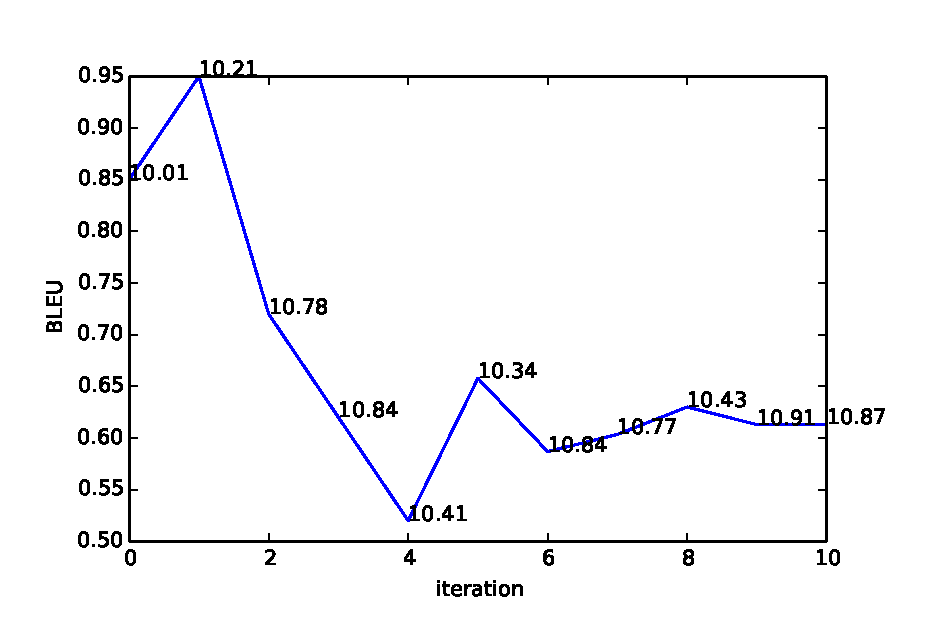
\includegraphics[width=0.45\textwidth]{Figures/condor_run.eps}
		\caption{Grid search over interpolation co-effs leading to a best BLEU of 10.91 using $\lambda_{d}$ = 0.612}
		\label{fig:condor}
	\end{figure}
	\begin{table*}
		\small
		\centering
		\begin{tabular}{p{0.5\textwidth}p{0.5\textwidth}p{0.6\textwidth}}
\toprule
Before & After & Reference \\ 
\toprule
\emph{her father y$\acute{a}$ng$\grave{a}$l$\acute{o}$$\grave{o}$ has l$\acute{a}$kw$\grave{e}$ everything} & the disease her father is not in a position to everything & the illness has rendered her father invalid \\
\midrule
\emph{the entrance of the child behind her back and let us go home} & the child behind her back and let us go home & take the baby in your back and let 's go home \\
\midrule
\emph{shaking/tension} & earthquake & earthquake \\
\bottomrule
\end{tabular} 
		\caption{Examples of improvements in translations}
		\label{table:examples}
	\end{table*}
		In the Table~\ref{table:examples}, we report examples of improvements in translations. In the first example, we observe that two words that were OOVs for our baseline model have translations after triangulation \& interpolation. In the second and third examples, we observe that triangulation leads to better translations. ``The entrance of the child'' is the only translation for the source phrase \emph{$l\acute{a}$} while after triangulation, we have several translations. In case of ``tranblemannt\`e'', our baseline model has several English translations but none of them mention ``earthquake''. They lead to shaking, tension, of the earthquake, but not the word ``earthquake''. 
	\subsection{Significance Tests}

		We report p-values obtained using multeval~\cite{Clark:11} comparing our best performing against two baselines. The results are reported in Table~\ref{table:significance}. We observe that our best system for Mawukakan and Maninkakan is significantly better than our baseline system, while the interpolated system with uniform weights achieves comparable performance to our best system. 

		On the other hand, our best system for Haitian Kreyol and Malagasy is not significant with p$<$0.05 compared to our baseline. However, it is significantly better than what we would have achieved had we used uniform weights. 
\end{comment}

\begin{comment}
\section{Related Work}
\label{sec:related_work}

	Previous research in triangulation share several characteristics. A large parallel corpora for source, pivot and target corpora derived from the same domain and languages which share several similarities (e.g vocabulary overlap). While~\cite{Utiyama:07} used multi-parallel Europarl comprising 560,000 sentences,~\cite{Cohn:07} used 700,000 multi-parallel europarl sentences, while a low-resource scenario was ``simulated'' by using the top10K sentences for each language.~\cite{Nakov:12} propose a language-independent approach to improving translation for low-resource languages, but the approach assumes the presence of a resource-rich language that bears similarity to the low-resource language, the similarities helping in creating a large triangulated phrase table. In~\cite{Nakovemnlp:12}, the resource-rich language is adapted to be more like the resource-poor one. Notice that this also assumes both are very similar. Results are reported using both Malay--Indonesian and Bulgarian--Macedonian, the third language being English in both cases.~\cite{Gispert:06} translate Catalan to Spanish via English by using news corpora on both source-pivot and pivot-target side.~\cite{Huck:12} report on BLEU score improvements by using $10^9$ parallel sentence between German and French.


	Consider a source language \emph{s}, pivot language \emph{p} and target language \emph{t}. When using the \emph{cascading} approach, we build two systems, between \emph{s} and \emph{p} and between \emph{p} and \emph{t}. Given a test set in \emph{s}, it is first translated to \emph{p} and those output translations are then translated into the target language \emph{t}. We do not report our results on using cascading for various reasons. Firstly, translating the output of a source-pivot system trained and tuned on little data will lead to propogation of errors. Secondly, we will need three development sets, one for each system.  Finally, it has been shown before that cascading does not give the most fluent translations.~\newcite{Utiyama:07} compared pivot-based triangulation with cascading using all of multi-parallel europarl, observing that pivot-based methods outperformed cascading.~\newcite{Bertoldi:08} compare and contrast various alignment heuristics that play a role in phrase extraction and propose a new way of random sampling of training data, reporting results on using triangulation for Chinese to Spanish via English.~\newcite{Wu:09} revisit the two approaches while also reporting results on using a synthetic approach. The datasets used are smaller in size compared to Europarl, released as part of IWSLT 2009, but, the design choices one needs to make when using pivot-based triangulation itself is not touched upon. Also, significant amount of monolingual data is used to expand the training data.
	

	The second approach is the pivot-based approach where a triangulated phrase table is generated between the source and target, by using the common pivot phrases between the source-pivot and pivot-target tables~\cite{Utiyama:07,Cohn:07}. Thus, the triangulated table largely depends on the number of target phrases in the source-pivot table. Having a very small source-pivot table leads to a relatively smaller triangulated table owing to the fewer number of common pivot phrases with the pivot-target system. Across all our experiments, the pivot-target system uses Europarl v7, comprising approximately 2 million parallel sentences. But our source-pivot for Maninkakan, Mawukakan, Haitian Kreyol and Malagasy has 4k, 5k, 30k and 30k parallel sentences respectively.~\newcite{Utiyama:07} observed that the triangulated table was able to achieve comparable BLEU scores to the direct system for French, German and Spanish. This could be owing to the fact that the data comprised multi-parallel 560K sentences.~\newcite{Cohn:07} observe that multiple pivot languages lead to more fluent translations compared to one pivot language. Multiple pivot language lead to multiple alternative translations, thus, increasing phrase coverage and rewarding the more appropriate translations and reducing out-of-vocabulary words further. They also propose a systematic way of combining the triangulated translation model with the direct model using linear interpolation and log-linear interpolation, although they assume a uniform weight for both the models.~\cite{Wu:09} compare~\cite{Utiyama:07} and~\cite{Cohn:07} but using data from a spoken language task. Moreover, the specific design choices one needs to make in pivot-based triangulation are not discussed. Finally, the data was in the same domain as well.~\cite{Bertoldi:08} propose using monolingual data more effectively and suggest sampling methods to improve the translations with triangulation. 

	To our best knowledge, Malagasy, Maninkakan and Mawukakan have not been studied before in the SMT literature. Although 9 systems participated in the workshop task on Haitian Kreyol, the approach of triangulation via French was not used.
\end{comment}

